\section{Widgets}

\begin{frame}[containsverbatim]{Container}

  \begin{figure}[h]
    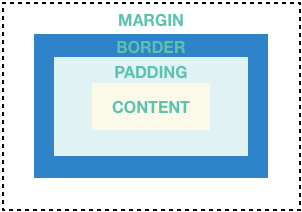
\includegraphics[width=0.25\textwidth]{images/margin-padding-border.png}
  \end{figure}

  \begin{minted}[fontsize=\footnotesize]{dart}
Container(
  margin: const EdgeInsets.all(10.0),
  color: Colors.amber[600],
  width: 48.0,
  height: 48.0,
);
	\end{minted}
  \footnotesize
  \url{https://api.flutter.dev/flutter/widgets/Container-class.html}
\end{frame}


\begin{frame}[containsverbatim]{Row}

  \begin{figure}[h]
    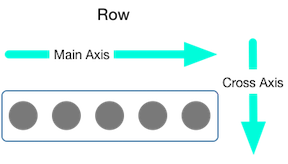
\includegraphics[width=0.25\textwidth]{images/row-diagram.png}
  \end{figure}

  \begin{minted}[fontsize=\footnotesize]{dart}
Row(
  mainAxisAlignment: MainAxisAlignment.spaceEvenly,
  children: [
    Image.asset('images/pic1.jpg'),
    Image.asset('images/pic2.jpg'),
    Image.asset('images/pic3.jpg'),
  ],
);
  \end{minted}
  \footnotesize
  \url{https://api.flutter.dev/flutter/widgets/Row-class.html}
\end{frame}

\begin{frame}[containsverbatim]{Column}

  \begin{figure}[h]
    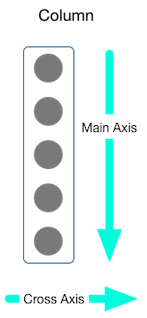
\includegraphics[height=0.25\textwidth]{images/column-diagram.png}
  \end{figure}

  \begin{minted}[fontsize=\footnotesize]{dart}
Column(
  mainAxisAlignment: MainAxisAlignment.spaceEvenly,
  children: [
    Image.asset('images/pic1.jpg'),
    Image.asset('images/pic2.jpg'),
    Image.asset('images/pic3.jpg'),
  ],
);
  \end{minted}
  \footnotesize
  \url{https://api.flutter.dev/flutter/widgets/Column-class.html}
\end{frame}

\begin{frame}[containsverbatim]{Text}

  \begin{minted}[fontsize=\footnotesize]{dart}
Text(
  'Hello, $_name! How are you?',
  textAlign: TextAlign.center,
  overflow: TextOverflow.ellipsis,
  style: const TextStyle(fontWeight: FontWeight.bold),
);
	\end{minted}
  \footnotesize
  \url{https://api.flutter.dev/flutter/widgets/Text-class.html}
\end{frame}

\begin{frame}[containsverbatim]{Elevated Button}

  \begin{minted}[fontsize=\footnotesize]{dart}
ElevatedButton(
  style: style,
  onPressed: () {print("Hello")},
  child: const Text('Click me'),
),
	\end{minted}
  \footnotesize
  \url{https://api.flutter.dev/flutter/material/ElevatedButton-class.html}
\end{frame}

\begin{frame}
  Now that we got that covered...
\end{frame}